\documentclass{article}\usepackage[]{graphicx}\usepackage[]{xcolor}
% maxwidth is the original width if it is less than linewidth
% otherwise use linewidth (to make sure the graphics do not exceed the margin)
\makeatletter
\def\maxwidth{ %
  \ifdim\Gin@nat@width>\linewidth
    \linewidth
  \else
    \Gin@nat@width
  \fi
}
\makeatother

\definecolor{fgcolor}{rgb}{0.345, 0.345, 0.345}
\newcommand{\hlnum}[1]{\textcolor[rgb]{0.686,0.059,0.569}{#1}}%
\newcommand{\hlstr}[1]{\textcolor[rgb]{0.192,0.494,0.8}{#1}}%
\newcommand{\hlcom}[1]{\textcolor[rgb]{0.678,0.584,0.686}{\textit{#1}}}%
\newcommand{\hlopt}[1]{\textcolor[rgb]{0,0,0}{#1}}%
\newcommand{\hlstd}[1]{\textcolor[rgb]{0.345,0.345,0.345}{#1}}%
\newcommand{\hlkwa}[1]{\textcolor[rgb]{0.161,0.373,0.58}{\textbf{#1}}}%
\newcommand{\hlkwb}[1]{\textcolor[rgb]{0.69,0.353,0.396}{#1}}%
\newcommand{\hlkwc}[1]{\textcolor[rgb]{0.333,0.667,0.333}{#1}}%
\newcommand{\hlkwd}[1]{\textcolor[rgb]{0.737,0.353,0.396}{\textbf{#1}}}%
\let\hlipl\hlkwb

\usepackage{framed}
\makeatletter
\newenvironment{kframe}{%
 \def\at@end@of@kframe{}%
 \ifinner\ifhmode%
  \def\at@end@of@kframe{\end{minipage}}%
  \begin{minipage}{\columnwidth}%
 \fi\fi%
 \def\FrameCommand##1{\hskip\@totalleftmargin \hskip-\fboxsep
 \colorbox{shadecolor}{##1}\hskip-\fboxsep
     % There is no \\@totalrightmargin, so:
     \hskip-\linewidth \hskip-\@totalleftmargin \hskip\columnwidth}%
 \MakeFramed {\advance\hsize-\width
   \@totalleftmargin\z@ \linewidth\hsize
   \@setminipage}}%
 {\par\unskip\endMakeFramed%
 \at@end@of@kframe}
\makeatother

\definecolor{shadecolor}{rgb}{.97, .97, .97}
\definecolor{messagecolor}{rgb}{0, 0, 0}
\definecolor{warningcolor}{rgb}{1, 0, 1}
\definecolor{errorcolor}{rgb}{1, 0, 0}
\newenvironment{knitrout}{}{} % an empty environment to be redefined in TeX

\usepackage{alltt}
\usepackage[sc]{mathpazo}
\renewcommand{\sfdefault}{lmss}
\renewcommand{\ttdefault}{lmtt}
\usepackage[T1]{fontenc}
\usepackage{geometry}
\geometry{verbose,tmargin=2.5cm,bmargin=2.5cm,lmargin=2.5cm,rmargin=2.5cm}
\setcounter{secnumdepth}{2}
\setcounter{tocdepth}{2}
\usepackage[unicode=true,pdfusetitle,
 bookmarks=true,bookmarksnumbered=true,bookmarksopen=true,bookmarksopenlevel=2,
 breaklinks=false,pdfborder={0 0 1},backref=false,colorlinks=false]
 {hyperref}
\hypersetup{
 pdfstartview={XYZ null null 1}}

\makeatletter
%%%%%%%%%%%%%%%%%%%%%%%%%%%%%% User specified LaTeX commands.
\renewcommand{\textfraction}{0.05}
\renewcommand{\topfraction}{0.8}
\renewcommand{\bottomfraction}{0.8}
\renewcommand{\floatpagefraction}{0.75}

\makeatother
\IfFileExists{upquote.sty}{\usepackage{upquote}}{}
\begin{document}



\title{}



\maketitle
The results below are generated from an R script.

\begin{knitrout}
\definecolor{shadecolor}{rgb}{0.969, 0.969, 0.969}\color{fgcolor}\begin{kframe}
\begin{alltt}
\hlcom{# Assignment: ASSIGNMENT 6}
\hlcom{# Name: Reppeto, Brian}
\hlcom{# Date: 2023-07-24}

\hlcom{## Set the working directory to the root of your DSC 520 directory}
\hlkwd{setwd}\hlstd{(}\hlstr{"~/DSC520/dsc520"}\hlstd{)}

\hlcom{## Load the `data/r4ds/heights.csv` to}
\hlstd{heights_df} \hlkwb{<-} \hlkwd{read.csv}\hlstd{(}\hlstr{"data/r4ds/heights.csv"}\hlstd{)}

\hlcom{## Load the ggplot2 library}
\hlkwd{library}\hlstd{(ggplot2)}

\hlcom{## Fit a linear model using the `age` variable as the predictor and `earn` as the outcome}
\hlstd{age_lm} \hlkwb{<-}  \hlkwd{lm}\hlstd{(}\hlkwc{formula} \hlstd{= earn} \hlopt{~} \hlstd{age,} \hlkwc{data} \hlstd{= heights_df)}

\hlcom{## View the summary of your model using `summary()`}
\hlkwd{summary}\hlstd{(age_lm)}
\end{alltt}
\begin{verbatim}
## 
## Call:
## lm(formula = earn ~ age, data = heights_df)
## 
## Residuals:
##    Min     1Q Median     3Q    Max 
## -25098 -12622  -3667   6883 177579 
## 
## Coefficients:
##             Estimate Std. Error t value Pr(>|t|)    
## (Intercept) 19041.53    1571.26  12.119  < 2e-16 ***
## age            99.41      35.46   2.804  0.00514 ** 
## ---
## Signif. codes:  0 '***' 0.001 '**' 0.01 '*' 0.05 '.' 0.1 ' ' 1
## 
## Residual standard error: 19420 on 1190 degrees of freedom
## Multiple R-squared:  0.006561,	Adjusted R-squared:  0.005727 
## F-statistic:  7.86 on 1 and 1190 DF,  p-value: 0.005137
\end{verbatim}
\begin{alltt}
\hlcom{## Creating predictions using `predict()`}
\hlstd{age_predict_df} \hlkwb{<-}
  \hlkwd{data.frame}\hlstd{(}\hlkwc{earn} \hlstd{=} \hlkwd{predict}\hlstd{(age_lm,} \hlkwc{newdata} \hlstd{= heights_df),} \hlkwc{age} \hlstd{= heights_df}\hlopt{$}\hlstd{age)}

\hlcom{## Plot the predictions against the original data}
\hlkwd{ggplot}\hlstd{(}\hlkwc{data} \hlstd{= heights_df,} \hlkwd{aes}\hlstd{(}\hlkwc{y} \hlstd{= earn,} \hlkwc{x} \hlstd{= age))} \hlopt{+}
  \hlkwd{geom_point}\hlstd{(}\hlkwc{color}\hlstd{=}\hlstr{'blue'}\hlstd{)} \hlopt{+}
  \hlkwd{geom_line}\hlstd{(}\hlkwc{color}\hlstd{=}\hlstr{'red'}\hlstd{,}\hlkwc{data} \hlstd{= age_predict_df,} \hlkwd{aes}\hlstd{(}\hlkwc{y}\hlstd{=earn,} \hlkwc{x}\hlstd{=age))}
\end{alltt}
\end{kframe}

{\centering 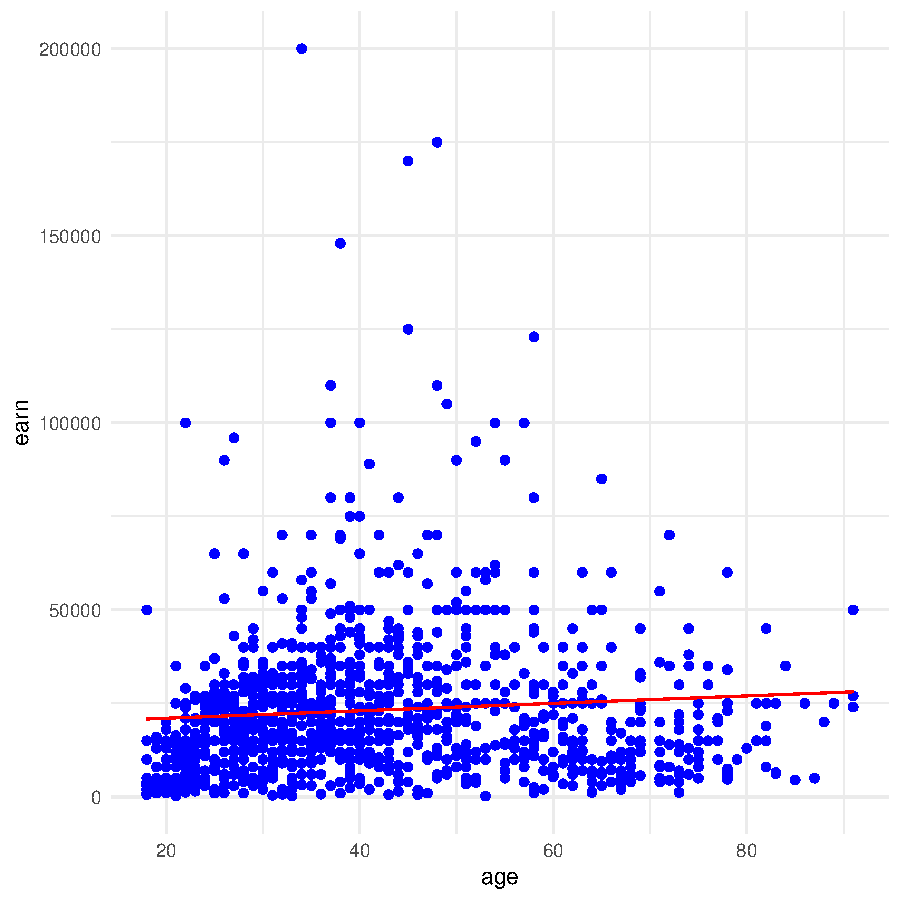
\includegraphics[width=.6\linewidth]{figure/assignment-06-ReppetoBrian-Rnwauto-report-1} 

}


\begin{kframe}\begin{alltt}
\hlstd{mean_earn} \hlkwb{<-} \hlkwd{mean}\hlstd{(heights_df}\hlopt{$}\hlstd{earn)}
\hlcom{## Corrected Sum of Squares Total}
\hlstd{sst} \hlkwb{<-} \hlkwd{sum}\hlstd{((mean_earn} \hlopt{-} \hlstd{heights_df}\hlopt{$}\hlstd{earn)}\hlopt{^}\hlnum{2}\hlstd{)}
\hlcom{## Corrected Sum of Squares for Model}
\hlstd{ssm} \hlkwb{<-} \hlkwd{sum}\hlstd{((mean_earn} \hlopt{-} \hlstd{age_predict_df}\hlopt{$}\hlstd{earn)}\hlopt{^}\hlnum{2}\hlstd{)}
\hlcom{## Residuals}
\hlstd{residuals} \hlkwb{<-} \hlstd{heights_df}\hlopt{$}\hlstd{earn} \hlopt{-} \hlstd{age_predict_df}\hlopt{$}\hlstd{earn}
\hlcom{## Sum of Squares for Error}
\hlstd{sse} \hlkwb{<-} \hlkwd{sum}\hlstd{(residuals}\hlopt{^}\hlnum{2}\hlstd{)}
\hlcom{## R Squared R^2 = SSM\textbackslash{}SST}
\hlstd{r_squared} \hlkwb{<-} \hlstd{ssm}\hlopt{/}\hlstd{sst}

\hlcom{## Number of observations}
\hlstd{n} \hlkwb{<-} \hlkwd{nrow}\hlstd{(heights_df)}
\hlcom{## Number of regression parameters}
\hlstd{p} \hlkwb{<-} \hlnum{2}
\hlcom{## Corrected Degrees of Freedom for Model (p-1)}
\hlstd{dfm} \hlkwb{<-} \hlstd{p}\hlopt{-}\hlnum{1}
\hlcom{## Degrees of Freedom for Error (n-p)}
\hlstd{dfe} \hlkwb{<-} \hlstd{n}\hlopt{-}\hlstd{p}
\hlcom{## Corrected Degrees of Freedom Total:   DFT = n - 1}
\hlstd{dft} \hlkwb{<-} \hlstd{n}\hlopt{-}\hlnum{1}

\hlcom{## Mean of Squares for Model:   MSM = SSM / DFM}
\hlstd{msm} \hlkwb{<-} \hlstd{sse}\hlopt{/}\hlstd{dfm}
\hlcom{## Mean of Squares for Error:   MSE = SSE / DFE}
\hlstd{mse} \hlkwb{<-} \hlstd{sse}\hlopt{/}\hlstd{dfe}
\hlcom{## Mean of Squares Total:   MST = SST / DFT}
\hlstd{mst} \hlkwb{<-} \hlstd{sst}\hlopt{/}\hlstd{dft}
\hlcom{## F Statistic F = MSM/MSE}
\hlstd{f_score} \hlkwb{<-} \hlstd{msm}\hlopt{/}\hlstd{mse}

\hlcom{## Adjusted R Squared R2 = 1 - (1 - R2)(n - 1) / (n - p)}
\hlstd{adjusted_r_squared} \hlkwb{<-} \hlnum{1} \hlopt{-} \hlstd{(}\hlnum{1} \hlopt{-} \hlstd{r_squared)}\hlopt{*}\hlstd{(n} \hlopt{-} \hlnum{1}\hlstd{)} \hlopt{/} \hlstd{(n} \hlopt{-} \hlstd{p)}

\hlcom{## Calculate the p-value from the F distribution}
\hlstd{p_value} \hlkwb{<-} \hlkwd{pf}\hlstd{(f_score, dfm, dft,} \hlkwc{lower.tail}\hlstd{=F)}
\end{alltt}
\end{kframe}
\end{knitrout}

The R session information (including the OS info, R version and all
packages used):

\begin{knitrout}
\definecolor{shadecolor}{rgb}{0.969, 0.969, 0.969}\color{fgcolor}\begin{kframe}
\begin{alltt}
\hlkwd{sessionInfo}\hlstd{()}
\end{alltt}
\begin{verbatim}
## R version 4.3.0 (2023-04-21)
## Platform: aarch64-apple-darwin20 (64-bit)
## Running under: macOS Ventura 13.4.1
## 
## Matrix products: default
## BLAS:   /System/Library/Frameworks/Accelerate.framework/Versions/A/Frameworks/vecLib.framework/Versions/A/libBLAS.dylib 
## LAPACK: /Library/Frameworks/R.framework/Versions/4.3-arm64/Resources/lib/libRlapack.dylib;  LAPACK version 3.11.0
## 
## locale:
## [1] en_US.UTF-8/en_US.UTF-8/en_US.UTF-8/C/en_US.UTF-8/en_US.UTF-8
## 
## time zone: America/New_York
## tzcode source: internal
## 
## attached base packages:
## [1] stats     graphics  grDevices utils     datasets  methods   base     
## 
## other attached packages:
##  [1] knitr_1.43       lm.beta_1.7-2    corrplot_0.92    lmtest_0.9-40    zoo_1.8-12      
##  [6] car_3.1-2        carData_3.0-5    conflicted_1.2.0 readxl_1.4.3     lubridate_1.9.2 
## [11] forcats_1.0.0    stringr_1.5.0    dplyr_1.1.2      purrr_1.0.1      readr_2.1.4     
## [16] tidyr_1.3.0      tibble_3.2.1     ggplot2_3.4.2    tidyverse_2.0.0 
## 
## loaded via a namespace (and not attached):
##  [1] utf8_1.2.3        generics_0.1.3    stringi_1.7.12    lattice_0.21-8   
##  [5] hms_1.1.3         magrittr_2.0.3    evaluate_0.21     grid_4.3.0       
##  [9] timechange_0.2.0  fastmap_1.1.1     cellranger_1.1.0  tinytex_0.45     
## [13] fansi_1.0.4       scales_1.2.1      abind_1.4-5       cli_3.6.1        
## [17] rlang_1.1.1       munsell_0.5.0     withr_2.5.0       cachem_1.0.8     
## [21] tools_4.3.0       tzdb_0.4.0        memoise_2.0.1     colorspace_2.1-0 
## [25] vctrs_0.6.3       R6_2.5.1          lifecycle_1.0.3   pkgconfig_2.0.3  
## [29] pillar_1.9.0      gtable_0.3.3      glue_1.6.2        highr_0.10       
## [33] xfun_0.39         tidyselect_1.2.0  rstudioapi_0.15.0 farver_2.1.1     
## [37] xtable_1.8-4      labeling_0.4.2    compiler_4.3.0
\end{verbatim}
\begin{alltt}
\hlkwd{Sys.time}\hlstd{()}
\end{alltt}
\begin{verbatim}
## [1] "2023-07-30 16:16:44 EDT"
\end{verbatim}
\end{kframe}
\end{knitrout}


\end{document}
